
\ctitle{Industriell bioteknologi}

\paragraph{Dette kapittelet} Del 1 beskriver hvordan celler responderer på endringer i omgivelsene. Del 2 forklarer metoder vi har for å få cellene til å lage kjemikalier vi ønsker oss. Del 3 er eksempler på industrielle produkter. Det siste eksempelet, antibiotika, er stort nok til å få sin egen del.

\cstitle{Adaptasjon}\index{adaptasjon}

\paragraph{Taktisk og strategisk adaptasjon} Vi skiller mellom to kategorier av mekanismer som celler har for å tilpasse seg endringer i miljøet. Kort og godt er forskjellen mellom dem at:
\begin{itemize}[nolistsep,noitemsep]
	\item Taktisk adaptasjon er \idx{endring i enzymaktivitet}: miljøet påvirker hvordan og i hvor stor grad et enzym fungerer.
	\item Taktisk adaptasjon går \emph{raskt}, gjerne i løpet av noen sekunder.
	\item Strategisk adaptasjon er \idx{endring i genuttrykk}: miljøet påvirker hvorvidt genet for et enzym uttrykkes.
	\item Strategisk adaptajon går \emph{tregt}, gjerne i løpet av timer eller dager.
\end{itemize}

\paragraph{Taktisk adaptasjon} Når cellen regulerer metabolismen ved å bruke enzymene som er tilgjengelig for å utføre reaksjonene som kreves der og da. Et eksempel på \ix{taktisk adaptasjon} er hvis produktet av en enzymdrevet reaksjon forhindrer enzymets funksjon, slik at konsentrasjonen av produktet kontrolleres ved negativ feedback.

\paragraph{Allosteriske enzymer}\index{allosterisk enzym} Proteiner som i tillegg til det aktive setet har et allosterisk sete med høy affinitet for bestemte små molekyler. Når slike molekyler er tilstede, forandrer de formen til proteinet slik at virkemåten forandres (det vil si at proteinet aktiveres eller deaktiveres). Det allosteriske setet trenger ikke å ligne på det aktive setet, så aktiviteten til allosteriske enzymer kan påvirkes av stoffer som ikke på noen måte ligner på substratet eller produktet til enzymet. Allosteriske enzymer representerer en type taktisk adaptasjon i celler.

Samtidig er mange enzymer laget av flere underenheter, der alle inneholder et aktivt sete og minst ett allosterisk sete. Disse enhetene er så tett bundet sammen at kjemisk binding på ett allosterisk sete vil forandre den romlige strukturen til både den gjeldende enheten og de andre enhetene. Denne koblingen mellom underenheter gjør det mulig å forsterke responsen på de hemmende eller aktiverende signalstoffene (altså stoffene som binder seg til de allosteriske setene) som organismen tar opp. Slike allosteriske enzymer fungerer som regulatorer i organismen, og har en viktig rolle flere steder i den metabolske prosessen.

For eksempel kan ett enkelt allosterisk ``pacemaker''-enzym i begynnelsen av prosessen bestemme takten på hele metabolismen. Et eksempel på dette er syntesen av glutamin i bakterier: når sluttproduktet akkumulerer i cellen, trigger det en \ix{negativ feedack}-mekanisme. Vi skal se i senere eksempler at negativ feedback i mikrober blir et problem når vi ønsker å bruke organismene til å produsere kjemikalier for oss.

\paragraph{Strategisk adaptasjon}\index{strategisk adaptasjon} Alle celler i en organisme inneholder den komplette genetiske informasjonen til organismen i DNA-et, men spesialiserte celler i høyere organismer trenger ikke å uttrykke alle genene i DNA-et. Derfor er mye av den genetiske informasjonen undertrykt, avhengig av celletype. Strategisk adaptasjon er cellens metoder for å uttrykke de genene det er ønskelig å uttrykke, og undertrykke resten av genene.

Også enkle organismer har strategisk adaptasjon. Enkelte bakterier, når de flyttes fra et vekstmedium med glukose til et medium der eneste sukkerart er \ix{laktose}, vil slutte å vokse (fordi de ikke har enzymene som kreves for å bryte ned laktose) i 20 minutter, før de begynner å vokse igjen (fordi de nå har klart å lage disse enzymene). Fenomenet, som kalles induksjon, skjer fordi laktose er en \ix{inducer} (kapittel 3, ``Strukturen til et gen'') som binder seg til \ix{repressorprotein}et som sitter på genet for laktosenedbrytende enzymer. Repressorproteinet endrer form slik at det ikke lenger sitter fast på DNA-et, og kan ikke lenger blokkere RNA polymerase fra å transkribere genene for laktosenedbrytende proteiner. Et tilsvarende eksempel er gjær, som beskrevet mot slutten av kapittel 1.

Å motvirke endringer i miljøet ved å midlertidig hemme hemmingen av syntesen av et enzym kalles, noe forvirrende, ``\ix{negativ kontroll}'', og må for all del ikke forveksles med negativ feedback.

Strategisk adaptasjon lar cellen bruke ressursene sine effektivt - for en bakterie ville det vært uøkonomisk å til enhver tid produsere alle enzymene den noensinne trenger, og for en høyere organisme er strategisk adaptasjon en absolutt nødvendighet (det hadde jo ikke vært så fint hvis nerveceller drev og produsere magesyre-enzymer).

\paragraph{Konstitutive enzymer}\index{konstitutivt enzym} Essensielle metabolske enzymer som alltid er til stede og produseres med en omtrentlig konstant rate.

\paragraph{Induserbare enzymer}\index{induserbart enzym} Enzymer som kun produseres når de trengs. Ellers er det repressorproteiner til stede som forhindrer at genet for det induserbare enzymet uttrykkes.

\cstitle{Industriell bioteknologi}\index{industriell bioteknologi}\index{hvit bioteknologi}
\paragraph{Industriell bioteknologi} Bioteknologi som brukes i industrielle prosesser. Også kjent som ``hvit bioteknologi''.

\paragraph{Black box model}\index{black box model} Den enkleste matematiske modellen av cellevekst, der alle cellereaksjoner grupperes sammen i én enkelt reaksjon, og cellen ses på som en ``svart boks'' der man ikke bryr seg om mekanismene for reaksjonen. En energikilde, en karbonkilde, en elektronakseptor og nitrogen går inn (energikilde og karbonkilde er som regel, men ikke alltid, den samme); cellen transformerer reaktantene; og biomasse, \ce{CO2}, vann og et metabolsk produkt kommer ut. Med denne modellen kan de 6 hovedtypene cellemetabolisme illustreres som i figur \ref{fig:blackbox}, hvor vi har henholdsvis
\begin{enumerate}[nolistsep,noitemsep]
	\item Fullstendig oksidasjon.
	\item Aerob cellevekst. Forholdet mellom karbon, hydrogen, nitrogen og oksygen i biomassen er 10:18:2:5.
	\item Aerob cellevekst med produktdannelse. Eksempel på produkt er glutamat.
	\item Anaerob cellevekst med produktdannelse. Eksempel på elektronakseptor er \ce{NO3}, eksempel på redusert elektronakseptor er \ce{NO2}.
	\item Fermentering: metabolisme i mangel av både oksygen og en elektronakseptor. Gir minimal cellevekst. Forskjellene mellom aerob metabolisme og fermentering ble beskrevet i kapittel 1.
	\item Crabtree-effekten (i gjær). Skjer når det er såpass overskudd av glukose at cellen må produsere etanol for å unngå intracellulær akkumulering av metabolitter.
\end{enumerate}
\begin{figure}[H]
	\centering
	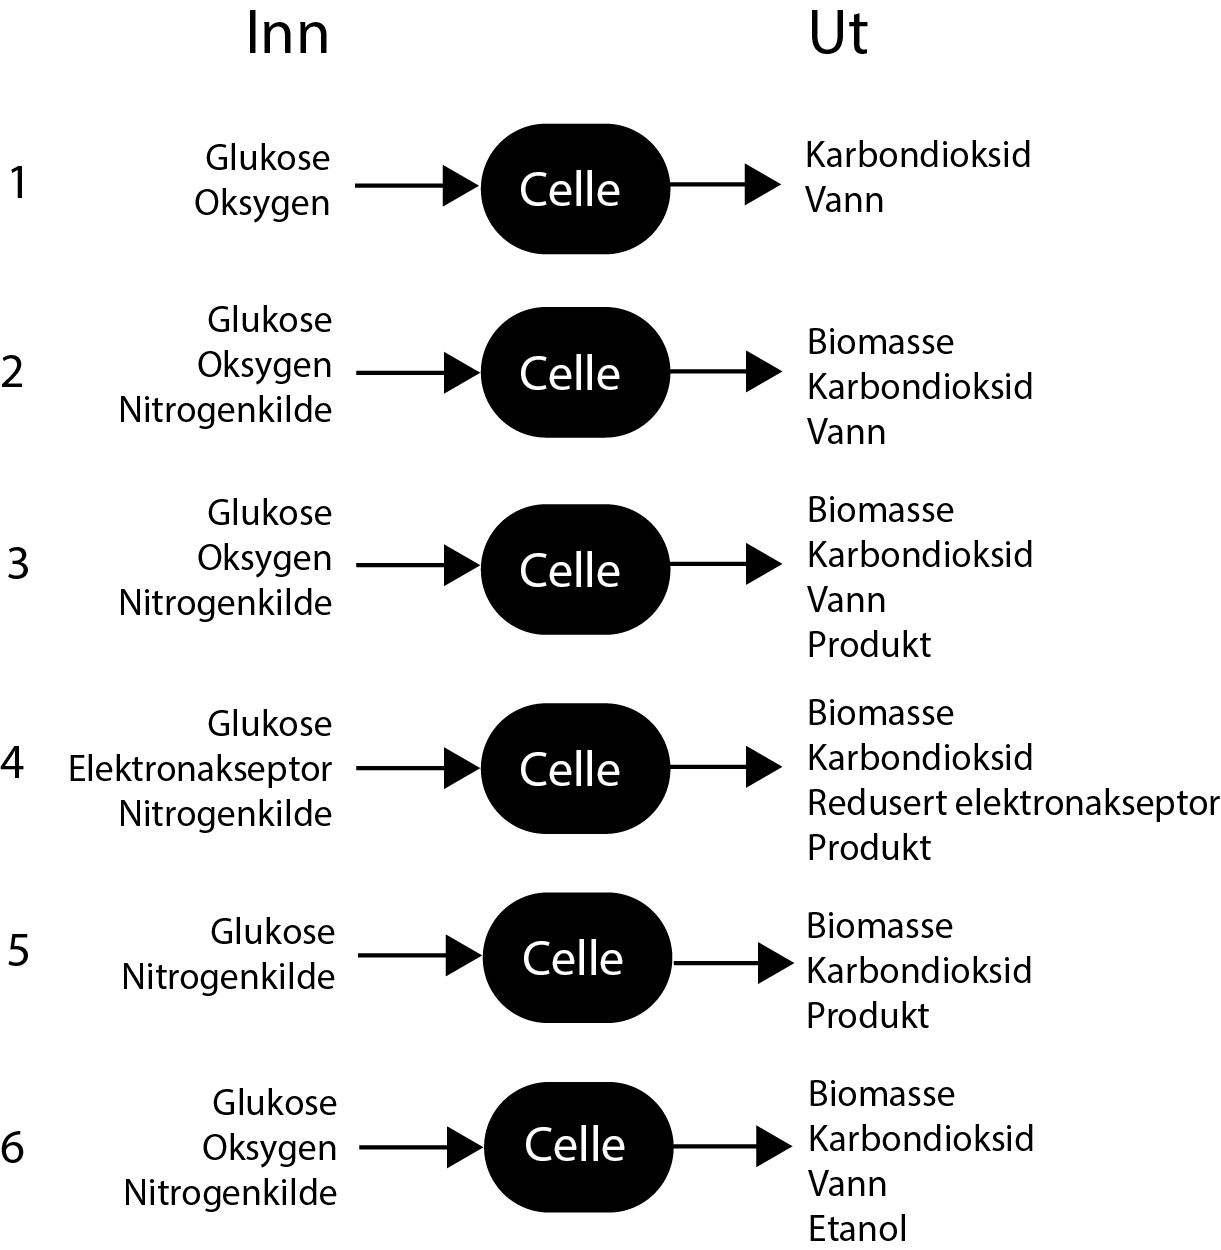
\includegraphics[width=0.45\textwidth]{blackbox}
	\caption{Forskjellige typer cellemetabolisme.}
	\label{fig:blackbox}
\end{figure}
I ``black box''-modellen anter vi at veksten i biomasse er proporsjonal med biomassen (altså enkel eksponensiell vekst). Proporsjonalitetskonstanten $\mu$ kalles \idx{spesifikk veksthastighet}, og er et resultat av at man dumper alle faktorer som kan påvirke veksthastigheten i én og samme parameter. Ligningen for biomassen blir
\begin{equation*}
	\frac{dm}{dt}=\mu m,
\end{equation*}
der $m$ er biomassen. Hvis biomassen er $m_0$ ved $t=0$, er løsningen på differensialligningen at
\begin{equation*}
	m=m_0e^{\mu t}.
\end{equation*}
Hvis vi måler tiden $t_d$ som det tar biomassen å fordoble seg, kan vi regne ut $\mu$. Siden $m=2m_0$ ved $t=t_d$, blir ligningen
\begin{equation*}
	2m_0=m_0e^{\mu t_d},
\end{equation*}
så
\begin{equation*}
	t_d=\frac{\ln 2}{\mu}\implies\mu=\frac{\ln 2}{t_d}.
\end{equation*}
En slik enkel modell har naturligvis sine begrensninger - for eksempel forutsier den at en \emph{E. coli}-bakterie med masse $m_0=3\times10^{-13}\text{ g}$ som deler seg etter $t_d=20\text{ min}$ (realistisk ved optimale vekstbetingelser) i løpet av 44 timer vil rekke å vokse til en koloni på størrelse med jordkloden.

\paragraph{Produktivitet} kan oppgis som total \ix{produktivitet} i milligram pr. sekund eller tonn pr. år; volumetrisk produktivitet som gram pr. liter pr. time; eller spesifikk produktivitet som gram pr. gram biomasse pr. time.

\paragraph{Utbytte}\index{utbytte} kan oppgis som gram biomasse pr. gram substrat; gram produkt pr. gram substrat; eller teoretisk maksutbytte, maks gram produkt pr. gram substrat.

\paragraph{Utvikling av bioprosesser}\index{utvikling av bioprosesser} Den tradisjonelle måten å utvikle organismer som produserer et kjemikalium man ønsker seg, kalles \ix{klassisk mutagenese} (``classical mutagenesis'') og består av følgende trinn:
\begin{enumerate}[nolistsep,noitemsep]
	\item Identifisere og isolere organismen som produserer det kjemikaliet man ønsker seg.
	\item Avle frem organismer med mutasjoner som fører til overproduksjon av produktet. Teknikker for å øke mutasjonsraten beskrives senere, i avsnittet om mutagener.
	\item Lab- og pilotprosjekt, der man finner optimale vekstforhold og slikt.
	\item Til slutt, produksjon på industriell og kommersiell skala.
\end{enumerate}
Alternativer til denne fremgangsmåten innebærer målrettet modifisering av DNA-et til en organisme for å frembringe det ønskede produktet (``\ix{metabolic engineering}'').

\paragraph{Bioreaktorer}\index{bioreaktor} Større ståltanker der man lager optimale vekstforhold for ønskelige mikrober ved å kontrollere
\begin{itemize}[nolistsep,noitemsep]
	\item Temperatur: høy temperatur steriliserer utstyret og forhindrer forurensning. Lav temperatur hindrer vekst av mikrober, men dreper dem ikke - derfor kan kulde brukes for å oppbevare mikroorganismer. 
	\item Trykk: høyt trykk inni reaktoren forhindrer forurensende organismer fra å komme inn i reaktoren. 
	\item Fuktighet: det finnes et optimalt fuktighetsnivå for mikroorganismene.
	\item pH: ved å kontrollere pH kan man forhindre vekst av uønskede mikrober og oppfordre til vekst av mikrobene man ønsker.
\end{itemize}

\cstitle{Eksempler}

\paragraph{Lysin}\index{lysin} Essensiell aminosyre som i naturen kun finnes i små mengder i korn. Man ønsker derfor å produsere lysin industrielt til f.eks dyrefôr. Lysin kan blant annet hentes fra \idx{Corynebacterium glutamicum}. For å få organismen til å produsere lysin i store mengder, må man forhindre negativ feedback: proteinet som lager lysin, aspartatkinase, blir deaktivert dersom det er både lysin og treonin til stede (treonin blir produsert litt senere i den metabolske prosessen via homoserin dehydrogenase). Hvis man finner en organisme med en mutasjon som forårsaker defekter i denne selvreguleringen, kan man produsere lysin i store mengder. To slike mutasjoner har blitt funnet: det finnes mutanter med
\begin{itemize}[nolistsep,noitemsep]
	\item en mutasjon i homoserin dehydrogenase forhindrer produksjon av treonin, slik at det alltid er lave treoninnivåer og aspartatkinase aldri blir deaktivert, og en med
	\item en mutasjon i aspartatkinase som gjør at det ikke deaktiveres av lysin. 
\end{itemize}

\paragraph{Glutamat}\index{glutamat} Aminosyre som kan brukes som tilsetning i mat for å få umami-smak. Glutamat dannes i sitronsyresyklusen. Den samme bakterien som ble brukt for produksjon av lysin, \idx{Corynebacterium glutamicum}, har en lite aktiv variant av enzymet oksoglutarat dehydrogenase. Dette ville forårsaket en opphopning av 2-oksoglutarat i cellen hvis det ikke hadde vært for et annet enzym, glutamat dehydrogenase, som konverterer 2-oksoglutarat til L-glutamat når det er ammoniumioner tilgjengelig. Ved å boble ammoniakk gjennom en bakteriekoloni kan man dermed produsere store mengder glutamat. Et siste problem er hvordan man får cellen til å skille ut glutamat i stedet for å la det hope seg opp i cellen. Løsningen kommer fra at bakterien ikke kan produsere biotin, en viktig komponent i cellevegger, men er avhengig av at det finnes i omgivelsene. Ved å gro bakteriene i et medium med minimale mengder biotin (akkurat nok til å tillate cellevekst) får man bakterier som slipper glutamat gjennom celeveggene. 

\paragraph{Mikrobiell produksjon av aminosyrer} Syntese via mikrober fungerer gjerne mye bedre enn kjemisk syntese hvis man skal produsere stereokjemisk komplekse molekyler, for eksempel biologiske aminosyrer som finnes i L-form som er biologisk aktiv og D-form som er biologisk inaktiv. Med kjemisk syntese ender man opp med rasemater - 50/50-blandinger av L- og D-formen, slik at halvparten av produktet er ubrukelig. Mikrobiell produksjon gir et produkt i 100\% L-form (siden enzymene i mikrobene er laget for å produsere L-formen).\index{D- og L-stereoisomeri}

\paragraph{Vitamin C}\index{vitamin C} Også kjent som L-askorbinsyre. Vitamin C kan ikke produseres av menneskekroppen og må derfor være i maten man spiser. Reichstein-metoden for å produsere Vitamin C er en \ix{kombinasjon av kjemisk syntese og bioteknologi} som består i å 
\begin{enumerate}[nolistsep,noitemsep]
	\item redusere D-glukose til D-sorbitol med nikkelkatalysator,
	\item la \emph{Acetobacter suboxydans} konvertere D-sorbitol til L-sorbose med sorbitol dehydrogenase (nesten 100\% effekt etter 2 dager), og til slutt
	\item kjemisk oksidere L-sorbose til 2-keto-L-gulonsyre, som i sur løsning danner L-askorbinsyre.
\end{enumerate}

\paragraph{Aspartam} Søtningsstoff som kan dannes av aspartat og fenylalanin, som begge produseres av bakterier eller med enzymer i bioreaktorer. Varer kun i 6-9 måneder, og er noget dyrere enn sakkarin og enzymprodusert fruktose - men hvis noen en dag finner en måte å bruke rekombinant genteknologi til å lage \ix{aspartam}produserende bakterier vil det trolig få en større markedsandel. Her er det gode muligheter, folkens.

\paragraph{Kortison}\index{kortison} Smertedempende stoff som kan produseres syntetisk med en komplisert prosess på 37 trinn, der noen av trinnene krever ekstreme forhold, til en pris på \$260 pr. gram. Ved å ta i bruk mikrobiell hydroksylering kan syntesen kuttes ned til 11 trinn som alle skjer ved normale betingelser, og prisen faller til \$1,30 pr. gram. 

Frem til 1975 hadde den meksikanske produsenten Proquivenex monopol på utgangsstoffet som ble brukt til å produsere kortison (diosgenin). Da de tidoblet prisen, svarte markedet ved å se etter alternative metoder som etter hvert erstattet den meksikanske råvaren, og markedet for diosgenin kollapset.

\cstitle{Antibiotika}
\paragraph{Penicillin}\index{penicillin} Etter at Alexander Fleming oppdaget penicillinens bakteriedrepende egenskaper, var det tre problemer som måtte løses for å kunne produsere penicillin billig og i store mengder:
\begin{enumerate}[noitemsep,nolistsep]
	\item Man måtte finne Penicillium-stammen som produserte mest penicillin.
	\item Man måtte finne en metode for å gro store mengder av bakterien.
	\item Man måtte finne en metode for å isolere penicillin fra vekstmediet.
\end{enumerate}
Det første problemet ble ``løst'' ved at man fant en svært effektiv penicillium-sopp på en cantaloupe i Peoria, Illinois - all sopp som brukes for å produsere penicillin i dag, er muterte etterkommere av denne soppen. Det andre og tredje problemet løses med bioreaktorer.

\paragraph{Mutagener}\index{mutagen}\index{mutasjon} For å finne sopp med mutasjoner som øker penicillin-produksjonen, ønsker man å øke mutasjonsraten - det er dessverre umulig å gjøre en målrettet mutasjon av bare ett gen, så man peiser på med mutasjoner og satser på at en av mutasjonene fungerer. Mutagener som øker mutasjonsraten inkluderer
\begin{itemize}[nolistsep,noitemsep]
	\item UV-stråling, som gjør at nabo-tymin i DNA dimeriserer.
	\item ioniserende stråling (røntgenstråler, gammastråler, nøytronstråler).
	\item diverse kjemikalier som reagerer med DNA-basene eller påvirker kopieringsprosessen.
\end{itemize}
Bruk av mutagener er en generell teknikk som er spesielt nyttig når man bare ønsker en mutasjon i ett gen. Det er litt verre med produksjon av sopp og bakterier som skal lage antibiotika, siden produksjonen avhenger av mange forskjellige gener. Derfor var det nødvendig med mange runder med seleksjon over et par tiår for å kunne gå fra penicilliumsoppen på cantaloupen i Peoria, til dagens penicillin-produsenter som produserer opp til 2000 ganger så mye penicillin. 

For å skape virkelig effektive organismer kan man avle frem flere forskjellige stammer parallelt, og etter flere generasjoner med kunstig seleksjon lage hybridorganismer av de forskjelilge datterkoloniene. Se boks 4.7.

Merk at superproduserende organismer ikke selv tjener noe på å lage en masse penicillin - de har bare dukket opp fordi \emph{mennesker} i hvert trinn har valgt ut organismene som tilfeldigvis produserte litt mer penicillin.

\paragraph{Virkemåten til penicillin} Penicillin dreper (Gram-negative) bakterier ved å forhindre produksjon av cellevegger. Dette gjør den ved å ha en $\beta$-laktamring som imiterer peptidbroa i celleveggen. Resultatet er at celleveggen blir så svak at cellen sprekker. 

\paragraph{Streptomycin og cephalosporiner} Alternative antibakterielle stoffer som er nødvendige for å drepe Gram-negative bakterier, samt Gram-positive bakterier som har blitt resistente til penicillin.  

\paragraph{Resistens}\index{resistens} Bakterier kan bli penicillin-resistente ved å produsere $\beta$-laktamaser som bryter ned $\beta$-laktamringen i penicillin. Som svar på dette har man laget nye semisyntetiske varianter av mikrobiell antibiotika, men hvert nye antibiotikum er bare en midlertidig løsning før det dukker opp nye bakterier som er resistente til dét også.

\paragraph{Hvorfor er overforbruk av antibiotika farlig?} Overforbruk av antibiotika vil føre til at resistente bakterier dannes, fordi man skaper et miljø der kun de antibiotikaresistente bakteriene overlever. Siden bakterier kan utveksle arvemateriale horisontalt via \ix{plasmid}er, vil et antibiotikaresistansgen kunne spre seg raskt gjennom bakteriekolonien.

\paragraph{Cyclosporin}\index{cyclosporin} I jakten på nye former for antibiotika oppdaget man at \idx{Tolypocladium inflatum} lager et ringformet peptid som, i tillegg til å være et OK antibiotikum, har en immundempende effekt. Peptidet, cyclosporin, var det første immundempende stoffet som ikke var så kraftig at det satte hele immunsystemet ute av spill. Cyclosporin binder seg spesifikt til visse reseptorer på T-celler og forhindrer reaksjonen av interleukin-2 (et signalmolekyl som setter i gang betennelsesreaksjoner). Oppdagelsen førte til en dramatisk økning i vellykkede organtransplantasjoner, fordi man på noenlunde kontrollert vis kunne forhindre immunsystemet i å avvise det transplanterte organet.
